% !TeX spellcheck = sv_SE
\documentclass[a4paper, 12pt]{report}

\usepackage[swedish]{babel}
\usepackage[T1]{fontenc}
\usepackage{lmodern}
\usepackage[utf8]{inputenc}

\usepackage{amsmath}
\usepackage{amssymb}
\usepackage{amsfonts}
\usepackage{amsthm}

\usepackage{graphicx}

\DeclareMathOperator{\sign}{sign}

\theoremstyle{definition}
\newtheorem{thm}{Sats}[section]
\newtheorem{lem}[thm]{Lemma}
\newtheorem{cor}[thm]{Korollarium}
\newtheorem{defi}{Definition}[section]
\newtheorem{ex}{Exempel}[section]
\theoremstyle{remark}
\newtheorem*{rem}{Observation}

\newtheorem*{reas}{Orsak}

\newcommand{\bfbeta}{{\boldsymbol{\beta}}}
\renewcommand\qedsymbol{$\blacksquare$}

\newcommand{\bfx}{\mathbf{x}}

\newcommand{\sephyp}{\{ \mathbf{x} : f(\mathbf{x})=\mathbf{x}^\intercal \bfbeta + \beta_0=0\}}

\newcommand{\entsephyp}{\{ \mathbf{x} : f(\mathbf{x})=\mathbf{x}^\intercal \bfbeta + \beta_0=0,~y_if(\mathbf{x}_i)\geq0,~i=1,\dots,~N,~\|\bfbeta\|=1\}}

\newcommand{\inprod}[2]{\langle \mathbf{#1}, \mathbf{#2}\rangle}

\title{Stödvektormaskiner\\
{\large Linjära hyperplan i Hilbertrum}}
\author{Oscar Granlund}


\begin{document}
\maketitle

\begin{abstract}
	Skrivs till sist
\end{abstract}

\chapter{Inledning}
Kort kapitel med avstamp i Vapniks ursprungliga algoritm för optimala separerande hyperplan (1963) och utvecklingen fram till 1995 då Vapnik och Cortes presenterade den första algoritmen med både mjuk marginal (Smith 1968, Bennet och Mangasarian 1992) och olinjära kärnor (Aizerman 1964, Poggio och Girosi 1990?) baserade på Aronszajns "Theory of Reproducing Kernels", 1950.

Hur uppsatsen relaterar till kapitlen om SVMs i boken "The Elements och Statistical Learning Theory".

\chapter{Stödvektormaskiner (SVM)}

\section{Klassificering med hjälp av separerande hyperplan}

\begin{defi}
	Ett \textit{klassificeringsproblem} är ett problem var man utgående från en mängd observationspar (\textit{träningsdata}) $(\mathbf{x}_i,y_i)$, $\mathbf{x}_i\in\mathbb{R}^p$, $y_i\in \{-1,1\}$, $i=1,\dots,~N$, försöker hitta en regel $g: \mathbb{R}^p \longmapsto \{-1,1\}$ sådan att $g(\mathbf{x}_i)=y_i$ för så många träningspar $(\mathbf{x}_i,y_i)$ som möjligt.
\end{defi}

Inom statistiken och maskininlärningen finns många olika metoder för att försöka lösa klassificeringsproblem, till exempel med hjälp av regressionsmodeller eller klusteranalys. I detta kapitel behandlas en metod där en affin mängd med dimensionen $p-1$ används för att definiera en regel som klassificerar \textit{observationerna} $\mathbf{x}_i$ i \textit{klasserna} $y_i\in\{-1,~1\}$ genom separering.

\begin{defi}
	Ett \textit{hyperplan} i ett vektorrum med dimensionen $p$ är ett underrum med dimensionen $p-1$, i figur \ref{fig:separatinghyperplane} illustreras ett separerande hyperplan för fallet $p=2$. Klassificeringsregeln $g$ för separerande hyperplan blir $g(\mathbf{x}_i)=\sign (\mathbf{x}_i^\intercal    \bfbeta + \beta_0)$ där mängden $\{\mathbf{x}: \mathbf{x}^\intercal \bfbeta + \beta_0=0\}$, med $\mathbf{x},~\bfbeta\in \mathbb{R}^p$, definierar ett hyperplan parametriserad av $\bfbeta$ och $\beta_0$.
\end{defi}

\begin{thm}\label{thm:hyperplan}
	Ett hyperplan definierat som den affina mängden $L=\sephyp$ har följande egenskaper \cite{ESL}:
	\begin{enumerate}
		\item $\bfbeta$ är en normalvektor till $L$ och kan normaliseras genom
		\begin{equation*}
			\widehat{\bfbeta} = \frac{\bfbeta}{\|\bfbeta\|}.
		\end{equation*}
		\item $\mathbf{x}_0^\intercal \bfbeta = -\beta_0$ för alla $\mathbf{x}_0$ i $L$.
		\item Det signerade avståndet från en punkt $\mathbf{x}$ till hyperplanet $L$, $\operatorname{d}^\pm (\mathbf{x}, L)$, ges av
		\begin{equation*}
		\begin{aligned}
			(\mathbf{x}-\mathbf{x}_0)^\intercal \widehat{\bfbeta} &= \frac{1}{\|\bfbeta\|}(\mathbf{x}^\intercal \bfbeta+\beta_0)\\
			&= \frac{1}{\|f^\prime(\mathbf{x})\|}f(\mathbf{x}).
		\end{aligned}
		\end{equation*}
	\end{enumerate}
\end{thm}
\begin{proof}
	\leavevmode
\begin{enumerate}
	\item Låt $\mathbf{x}_1$ och $\mathbf{x}_2$ vara två punkter i $L$. Då gäller att $f(\mathbf{x}_1)=f(\mathbf{x}_2)=0$ och
	\begin{align*}
		0 &= f(\mathbf{x}_1)-f(\mathbf{x}_2)\\
		&= \mathbf{x}_1^\intercal \bfbeta + \beta_0 - \mathbf{x}_2^ \intercal \bfbeta - \beta_0\\
		&= (\mathbf{x}_1-\mathbf{x}_2)^\intercal \bfbeta
	\end{align*}
	alltså uppfyller $\bfbeta$ kravet för normalvektorer och $\widehat{\bfbeta}:=\frac{\bfbeta}{\|\bfbeta\|}$ är den normaliserade normalvektorn till hyperplanet $L$. \hfill\qedsymbol
	\item \label{eq:egenskap2}Låt $\mathbf{x}_0$ vara en punkt i $L$. Då gäller att $f(\mathbf{x}_0)=\mathbf{x}_0^\intercal \bfbeta + \beta_0 = 0$ alltså är $\mathbf{x}^\intercal_0 \bfbeta = - \beta_0$.\hfill \qedsymbol
	\item Låt $\mathbf{x}_0$ vara en punkt i hyperplanet $L$. Då är avståndet från hyperplanet till punkten $\mathbf{x}$ lika med längden av projektionen av vektorn $(\mathbf{x}-\mathbf{x}_0)$ på hyperplanets normaliserade normal $\widehat{\beta}$, $\operatorname{comp_{\widehat{\bfbeta}}} ( \mathbf{x} - \mathbf{x}_0 )$. Vi får alltså att
	\begin{align*}
		\operatorname{d^\pm} ( \mathbf{x}, L ) &= \operatorname{comp_{\widehat{\bfbeta}}} ( \mathbf{x} - \mathbf{x}_0 )
		=\underline{\underline{ (\mathbf{x} - \mathbf{x}_0)^\intercal \widehat{\bfbeta} }}\\
		&= \frac{1}{\|\bfbeta\|}(\mathbf{x}^\intercal\bfbeta - \mathbf{x}_0^\intercal\bfbeta)=\underline{\underline{\frac{1}{\|\bfbeta\|}(\mathbf{x}^\intercal\bfbeta + \beta_0)}}
	\end{align*}
	där det sista steget följer från egenskap \ref{eq:egenskap2} då $\mathbf{x}_0$ är en punkt i $L$. Om man vidare noterar att $f(\mathbf{x})=\mathbf{x}^\intercal\bfbeta+\beta_0$ och $f^\prime(\mathbf{x})=\bfbeta$ så fås även att
	\begin{equation*}
		\frac{1}{\|\bfbeta\|}(\mathbf{x}^\intercal\bfbeta + \beta_0)=\frac{1}{\|f^\prime(\mathbf{x})\|}f(\mathbf{x}).
	\end{equation*}
	\qedhere
\end{enumerate}
\end{proof}

\begin{rem}
	Definitionen $L=\{ \mathbf{x} : f(\mathbf{x})=\mathbf{x}^\intercal \bfbeta + \beta_0=0\}$ för hyperplanet $L$ är inte entydig.
\end{rem}
\begin{reas}
	Betrakta hyperplanen $L_1 = \sephyp$ och $L_2 = \left\{\mathbf{x}: g(\mathbf{x})=\mathbf{x}^\intercal(-\bfbeta) + (-\beta_0) = 0\right\}$. Eftersom att $g(\mathbf{x}) = -f(\mathbf{x})$ så gäller att om $\mathbf{x}_0$ tillhör $L_1$ så tillhör $\mathbf{x}_0$ även $L_2$.
	Betrakta vidare hyperplanet $L_3= \left\{\mathbf{x}: h(\mathbf{x})=\frac{\mathbf{x}^\intercal\bfbeta}{\|\bfbeta\|} + \frac{\beta_0}{\|\bfbeta\|}=0\right\}$. Om $\mathbf{x}_0$ då tillhör $L_1$ så tillhör $\mathbf{x}_0$ även $L_3$ eftersom att $h(\mathbf{x}) = \frac{f(\mathbf{x})}{\|\bfbeta\|}=0$. Notera även att $\frac{1}{\|\bfbeta\|}$ kunde ha varit vilket reellt tal som helst.
\end{reas}

\begin{rem}
	För att få entydiga hyperplan för klassificering kan man lägga till villkor. Om man kräver att $\|\bfbeta\|=1$ och $y_i(\mathbf{x}_i^\intercal\bfbeta + \beta_0)\geq0$ för alla $i=1,\dots,~N$, där $y_i$ är klasserna i klassificeringsproblemet, så får man en entydig definition av hyperplanet där vektorn $\bfbeta$ ''pekar mot`` klassen där $y_i=1$ och $\beta_0$ anger det signerade avståndet (i relation till riktningen på $\bfbeta$) från origo till hyperplanet.
\end{rem}
\begin{reas}
	De extra villkoren gör att man inte längre kan göra manipulationerna som påvisade icke-entydigheten. Om man sätter $\mathbf{x}=\mathbf{0}$ så får man med hjälp av sats \ref{thm:hyperplan} att avståndet från origo till planet är lika med $\frac{1}{\|\bfbeta\|}(\mathbf{x}^\intercal\bfbeta+\beta_0)=\frac{1}{\|\bfbeta\|}\left(\mathbf{0}^\intercal\bfbeta+\beta_0\right)=\beta_0$.
\end{reas}

\begin{figure}[h]
\centering
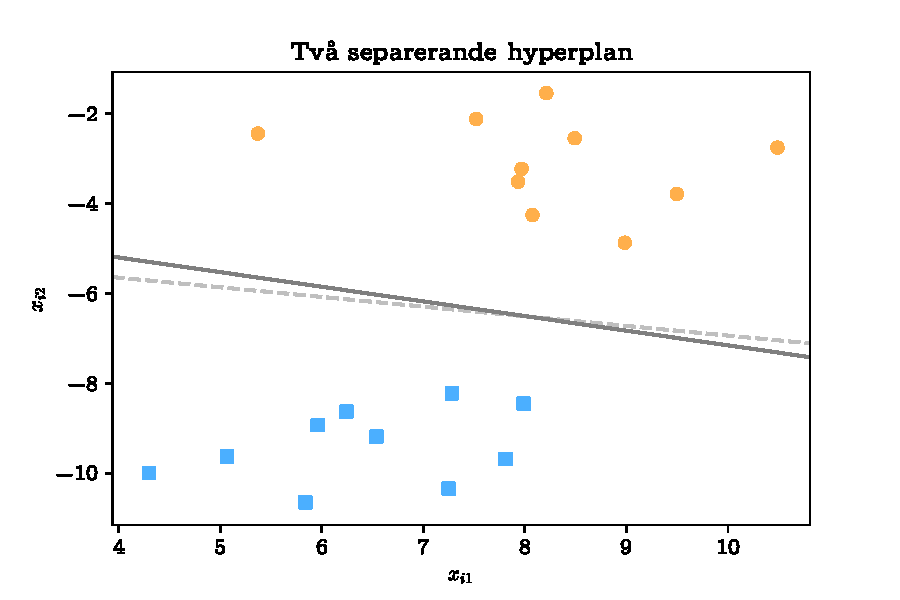
\includegraphics[width=0.8\linewidth, trim={0.5cm 2mm 0.5cm 6mm}, clip]{KandFigur1.pdf}
\caption{\label{fig:separatinghyperplane}20 datapunkter med två separerande hyperplan (linje) där klassen $y_i=1$ framställs som blå fyrkanter och klassen $y_i=-1$ som orangea cirklar.}
\end{figure}

\begin{defi}
	Ett klassificeringsproblem eller en mängd observationspar $\left(\mathbf{x}_i, y_i\right)$ är \textit{linjärt separabelt} om det existerar ett hyperplan $L=\sephyp$ som separerar klasserna.
\end{defi}

%TODO SKRIVA OM SATS OCH BEVIS ENLIGT BOYD
\begin{thm} \cite{Boyd}
	För ett hyperplan $L=\sephyp$ som separerar två klasser gäller att
	\begin{equation*}
		y_i(\mathbf{x}_i^\intercal \bfbeta + \beta_0) > 0
	\end{equation*}
	eller
	\begin{equation*}
		y_i(\mathbf{x}_i^\intercal \bfbeta + \beta_0) < 0
	\end{equation*}
	för alla $i = 1, \dots,~N$.
\end{thm}
\begin{proof}
	Ifall ett klassificeringsproblem är linjärt separabelt så ligger alla observationer $y_i$ på rätt sida av hyperplanet definierat genom $\mathbf{x}^\intercal \bfbeta + \beta_0$; eller så ligger alla observationer på fel sida av hyperplanet. Vilket betyder att ifall $y_i=1$ så är $\mathbf{x}_i^\intercal \bfbeta + \beta_0 > 0$ och om $y_i=-1$ så är $\mathbf{x}_i^\intercal \bfbeta + \beta_0 < 0$. Detta betyder att $y_i(\mathbf{x}_i^\intercal \bfbeta + \beta_0) > 0$. Ifall $\mathbf{x}_i^\intercal \bfbeta + \beta_0 = 0$ är problemet inte linjärt separabelt.
\end{proof}

\begin{ex}\label{exempel:mångahyperplan}
	Låt observationsparen vara $(\left[2,~2\right]^\intercal,~1),~(\left[1,~2\right]^\intercal,-1)$. Då är $$L_1=\{\mathbf{x}\in\mathbb{R}^2: \mathbf{x}^\intercal\begin{bmatrix}
	1\\
	0
	\end{bmatrix} - 1.5=0\}$$ och $$L_2=\{\mathbf{x}\in\mathbb{R}^2: \mathbf{x}^\intercal\begin{bmatrix}
	\sqrt{2}\\
	\sqrt{2}
	\end{bmatrix} - 3.5\sqrt{2}=0\}$$ två separerande hyperplan (linjer i detta fall).
\end{ex}
\begin{proof}
	För $L_1$: $$y_1(\mathbf{x}_1^\intercal\begin{bmatrix}
	1\\
	0\end{bmatrix}-1.5)=\left[2,~2\right]^\intercal\begin{bmatrix}
	1\\
	0\end{bmatrix}-1.5=0.5>0$$ och $$y_2(\mathbf{x}_2^\intercal\begin{bmatrix}
	1\\
	0\end{bmatrix}-1.5)=-1(\left[1,~2\right]^\intercal\begin{bmatrix}
	1\\
	0\end{bmatrix}-1.5)=(-1)(-0.5)=0.5>0.$$
	Och för $L_2$: $$y_1(\mathbf{x}_1^\intercal\begin{bmatrix}
	\sqrt{2}\\
	\sqrt{2}\end{bmatrix}-3.5\sqrt{2})=\left[2,~2\right]^\intercal\begin{bmatrix}
	\sqrt{2}\\
	\sqrt{2}\end{bmatrix}-3.5\sqrt{2}=0.5\sqrt{2}>0$$ och $$y_2(\mathbf{x}_2^\intercal\begin{bmatrix}
	\sqrt{2}\\
	\sqrt{2}\end{bmatrix}-3.5\sqrt{2})=-1(\left[1,~2\right]^\intercal\begin{bmatrix}
	\sqrt{2}\\
	\sqrt{2}\end{bmatrix}-3.5\sqrt{2})=(-1)(-0.5\sqrt{2})=0.5\sqrt{2}>0$$
\end{proof}

\begin{rem}
	Hyperplan kan konstrueras enkelt genom att man i $\mathbb{R}^p$ väljer $p$ stycken punkter $\mathbf{x}_i$ som man vill att planet ska gå igenom, sedan löser man ekvationssystemet $X\bfbeta=-\beta_0\mathbf{1}$, i vilket $X$ är en matris där raderna består av punkterna $\mathbf{x}_i$, $i=1,\dots, p$, och $\beta_0\mathbf{1}$ är en vektor med värdet $\beta_0$ i alla rader.
\end{rem}

Som syns i exempel \ref{exempel:mångahyperplan} finns det många separerande hyperplan om ett klassificeringsproblem är linjärt separabelt och frågan är då vilket separerande hyperplan man borde välja.

\section{Optimala separerande hyperplan}
Inom statistiken finns många olika metoder som en modell till data och metoderna kan ofta visas vara ekvivalenta med något optimeringsproblem, till exempel maximum likelihood-metoden (ML-metoden) för linjär regression, som är ekvivalent med minstakvadratmetoden. %TODO% REFERENS 
Optimeringsproblemen kan oftast ändras genom att man lägger till eller tar bort termer i objektivfunktionen eller ändrar på kraven.

För separerande hyperplan kommer jag att behandla ett optimeringsproblem som är utformat så att det kortaste avståndet från hyperplanet till de närmaste observationsparen från vardera klass maximeras \cite{Vapnik96}. Med andra ord fås följande optimeringsproblem
\begin{equation}\label{opt:optimalmargin1}
\begin{aligned}
	 \operatornamewithlimits{max}_{\widehat{\bfbeta},\widehat{\beta}_0,\|\widehat{\bfbeta}\|=1}& & &C\\
	 \text{så att}& & &y_i(\mathbf{x}_i^\intercal\widehat{\bfbeta}+\widehat{\beta}_0)\geq C,\quad i=1,\dots,N
\end{aligned}
\end{equation}
där $C$ kallas \emph{marginalen} och betecknar avståndet från hyperplanet till de närmaste punkterna.
\begin{rem}
	Ifall alla punkter är rätt klassificerade så anger $y_i(\mathbf{x}^\intercal_i\widehat{\bfbeta}+\widehat{\beta}_0)$ det absoluta avståndet mellan hyperplanet och punkten $\mathbf{x}_i$.
\end{rem}

Förhoppningen är att om man väljer det separerande hyperplan som befinner sig så långt som möjligt från båda klasserna får ett hyperplan som även generaliserar väl till ny data. Dessutom är detta även ett unikt sätt att välja ett separerande hyperplan det vill säga optimeringsproblemet är konvext.

För att visa att optimeringsproblemet (\ref{opt:optimalmargin1}) är \textit{konvext} måste det skrivas om. Idén är här att man låter inversen av längden på vektorn $\bfbeta$ beskriva avståndet till närmast punkt. På så sätt skapas en direktare länk mellan kraven och objektfunktionen i optimeringsproblemet.

Först måste alltså kravet $\|\widehat{\bfbeta}\|=1$ bytas ut. Detta görs genom att man byter ut kraven
\begin{equation*}
y_i(\mathbf{x}_i^\intercal\widehat{\bfbeta}+\widehat{\beta}_0)\geq C,\quad i=1,\dots,N
\end{equation*}
mot kraven
\begin{equation*}
y_i\left(\mathbf{x}_i^\intercal\frac{\bfbeta}{\|\bfbeta\|}+\frac{\beta_0}{\|\bfbeta\|}\right) = 
\frac{1}{\|\bfbeta\|}y_i(\mathbf{x}_i^\intercal\bfbeta+\beta_0)
 \geq C,\quad i=1,\dots,N
\end{equation*}
eller ekvivalent
\begin{equation*}
y_i(\mathbf{x}_i^\intercal\bfbeta+\beta_0)\geq C\|\bfbeta\|,\quad i=1,\dots,N,
\end{equation*}
där man valt en av de andra representationerna för samma hyperplan genom att skala om $\widehat{\bfbeta}$ och $\widehat{\beta}_0$. Vidare kan $C$ elimineras genom att man väljer $C=\frac{1}{\|\bfbeta\|}$, då fås
\begin{equation*}
y_i(\mathbf{x}_i^\intercal\bfbeta+\beta_0)\geq 1,\quad i=1,\dots,N
\end{equation*}
och eftersom $C=\frac{1}{\|\bfbeta\|}$ är en avtagande funktion med avseende på $\|\bfbeta\|$ är maximering av $C$ ekvivalent med minimering av $\|\bfbeta\|$ och motsvarande optimeringsproblemet blir
\begin{equation*}%\label{opt:optimalmargin2}
\begin{aligned}
\operatornamewithlimits{min}_{\bfbeta,\beta_0} & & &\|\bfbeta\|\\
\text{så att} & & &y_i(\mathbf{x}_i^\intercal\bfbeta+\beta_0)\geq 1,\quad i=1,\dots,N.
\end{aligned}
\end{equation*}
Därefter görs ännu en konvexitetsbevarande kvadratisk transformering av \textit{kostfunktionen} $\|\bfbeta\|$, det vill säga man noterar att \begin{equation*}
\operatornamewithlimits{argmin}_{\bfbeta,\beta_0} \|\bfbeta\|=\operatornamewithlimits{argmin}_{\bfbeta,\beta_0} \frac{1}{2}\|\bfbeta\|^2.
\end{equation*}
En orsak till att göra den kvadratiska transformeringen är att man på så sätt kan garantera att objektfunktionen är deriverbar:
\begin{ex}
	Låt $f(x):=|x-x_0|$ och $g(x):=\left(f(x)\right)^2$. Då är $f(x)$ inte deriverbar i punkten $x_0$ medan $D_x\left(g(x)\right)=D_x\left(\left(x-x_0\right)^2\right)=D_x\left(x^2-2xx_0+x_0^2\right)=2x-2x_0=2(x-x_0)$ och $D_x\left(g(x_0)\right)=0$ det vill säga $\operatornamewithlimits{argmin}_x f(x) = x_0 = \operatornamewithlimits{argmin}_x g(x)$.
\end{ex}
Optimeringsproblemet \ref{opt:optimalmargin1} kan alltså skrivas på formen 
\begin{equation*}
\begin{aligned}
\operatornamewithlimits{min}_{\bfbeta,\beta_0} & & &\frac{1}{2}\|\bfbeta\|^2=\frac{1}{2}\bfbeta^\intercal\bfbeta=\bfbeta^\intercal\left(\frac{1}{2}I\right)\bfbeta\\
\text{så att} & & &y_i(\mathbf{x}_i^\intercal\bfbeta+\beta_0)\geq 1,\quad i=1,\dots,N
\end{aligned}
\end{equation*}
där $\left( \frac{1}{2}I \right)$ är en \emph{positiv semi-definit} matris det vill säga den uppfyller kraven för att ett kvadratiskt optimeringsproblem med linjära lösbara krav ska vara konvext \cite{Boyd}.

\begin{rem}
	För två vektorer $\mathbf{a}$ och $\mathbf{b}$ i $\mathbb{R}^p$ kan produkten $\mathbf{a}^\intercal\mathbf{b}$ uttryckas som den normala inre produkten $\langle \mathbf{a}, \mathbf{b} \rangle$ i $\mathbb{R}^p$. Detta kommer till nytta i kapitel \ref{chap:hilbert} där konvexiteten för en generalisering av det linjära problemet utforskas.
\end{rem}

Ovanstående resonemang är ett bevis för sats \ref{thm:primallinearproblem}.
\begin{thm}\label{thm:primallinearproblem}
	Låt $\widehat{\bfbeta},~\bfbeta \in \mathbb{R}^p$ och $\widehat{\beta}_0,~\beta_0 \in \mathbb{R}$. Låt dessutom observationsparen $\left(\mathbf{x}_i, y_i\right)$ vara linjärt separabla. Då är optimeringsproblemet
	\begin{equation*}
	\begin{aligned}
	\operatornamewithlimits{max}_{\widehat{\bfbeta},\widehat{\beta}_0,\|\widehat{\bfbeta}\|=1} & & &C\\
	\text{så att} & & &y_i(\mathbf{x}_i^\intercal\widehat{\bfbeta}+\beta_0)\geq C,\quad i=1,\dots,N
	\end{aligned}
	\end{equation*}
	konvext och ekvivalent med optimeringsproblemet %TODO är kanske inte ekvivalent?
	\begin{equation*}
	\begin{aligned}
	\operatornamewithlimits{min}_{\bfbeta,\beta_0} & & &\frac{1}{2}\|\bfbeta\|^2\\
	\text{så att} & & &y_i(\mathbf{x}_i^\intercal\bfbeta+\beta_0)\geq 1,\quad i=1,\dots,N.
	\end{aligned}
	\end{equation*}
\end{thm}
Vidare ger observationen ovan ytterligare ett ekvivalent optimeringsproblem:
\begin{cor}\label{cor:inreproduktoptimering}
	Optimeringsproblemen i sats \ref{thm:primallinearproblem} är ekvivalenta med optimeringsproblemet
	\begin{equation*}
	\begin{aligned}
	\operatornamewithlimits{min}_{\bfbeta,\beta_0} & & &\frac{1}{2}\langle \bfbeta, \bfbeta \rangle\\
	\text{så att} & & &y_i(\langle \mathbf{x}_i,\bfbeta\rangle+\beta_0)\geq 1,\quad i=1,\dots,N
	\end{aligned}
	\end{equation*}
	med samma antaganden.
\end{cor}
\begin{proof}
	Normen $\|\bfbeta\|=(\bfbeta^\intercal\bfbeta)^{\frac{1}{2}}$ kan uttryckas som $\langle \bfbeta, \bfbeta \rangle^{\frac{1}{2}}$ alltså är $\frac{1}{2} \|\bfbeta\|^2=\frac{1}{2}\langle \bfbeta, \bfbeta \rangle$. Resten följer från observationen.
\end{proof}
Framställningen i korollarium \ref{cor:inreproduktoptimering} används i många källor, bland annat i den ursprungliga framställningen för stödvektormaskinen, %TODO referens
och är en av de mer generella framställningarna för optimeringsproblemet som stödvektormaskinen bygger på. %TODO Ha kvar dethär?

\subsection{Primala och duala problem}

För att hitta alla extrempunkter till ett optimeringsproblem, det vill säga lösa ett konvext optimeringsproblem, används Lagrangemultiplikatorer \cite{Boyd}.
Den primala Lagrangefunktionen $L_P$ för optimeringsproblemet
\begin{equation*}
\begin{aligned}
\operatornamewithlimits{min}_{\bfbeta,\beta_0} & & &\frac{1}{2}\|\bfbeta\|^2\\
\text{så att} & & &y_i(\mathbf{x}_i^\intercal\bfbeta+\beta_0)\geq 1,\quad i=1,\dots,N
\end{aligned}
\end{equation*}
ges då av
\begin{equation}\label{eq:primallagrange}
L_P=\frac{1}{2}\|\bfbeta\|^2 - \sum_{i=1}^{N} \lambda_i\left(y_i \left(\mathbf{x}_i^\intercal\bfbeta + \beta_0\right)-1\right)
\end{equation}
som ska minimeras med avseende på $\bfbeta$ och $\beta_0$.

För att minimera $L_P$ sätts derivatorna med avseende på elementen $\left[\bfbeta\right]_j$ av $\bfbeta$ och $\beta_0$ till 0, och följande relationer erhålls:
\begin{equation}\label{eq:derivprimal}
\begin{aligned}
	D_{ \left[\bfbeta\right]_j } (L_P) &= D_{ \left[\bfbeta\right]_j } \left( \frac{1}{2} \bfbeta^\intercal \bfbeta \right) &- &D_{ \left[\bfbeta\right]_j } \left( \sum_{i=1}^{N} \left( \lambda_i y_i \left( \mathbf{x}_i^\intercal\bfbeta \right) + \lambda_i y_i \beta_0 - \lambda_i \right)\right)\\
	&= D_{ \left[\bfbeta\right]_j } \left( \frac{1}{2} \sum_{k=1}^{p} \left[\bfbeta\right]_k^2 \right) &- &\sum_{i=1}^{N} D_{ \left[\bfbeta\right]_j } \left(  \lambda_i y_i \left(\sum_{k=1}^{p}\left[\mathbf{x}_i\right]_k\left[\bfbeta\right]_k \right) + \lambda_i y_i \beta_0-\lambda_i \right)\\
	&= [\bfbeta]_j &- &\sum_{i=1}^{N} D_{ \left[\bfbeta\right]_j } \left( \sum_{k=1}^{p} \lambda_i y_i \left[\mathbf{x}_i\right]_k\left[\bfbeta\right]_k \right) + 0\\
	&= [\bfbeta]_j &- &\sum_{i=1}^{N}\lambda_i y_i \left[ \mathbf{x}_i \right]_j
\end{aligned}
\end{equation}
där $j=1,\dots p$ och
\begin{equation*}
	D_{\beta_0}(L_P) = D_{\beta_0}\left( -\sum_{i=1}^{N} \lambda_i y_i \beta_0 \right) = -\sum_{i=1}^{N} \lambda_i y_i.
\end{equation*}
Vidare kan (\ref{eq:derivprimal}) skrivas om som derivatan med avseende på hela $\bfbeta$ eftersom att $ \left[ D_{ \bfbeta }(L_p) \right]_j = D_{\left[ \bfbeta \right]_j}(L_p) $. Efter att man tar i beaktande kraven att $ D_{ \bfbeta }(L_p) = \mathbf{0} $ och $ D_{\beta_0}(L_p)=0 $ fås följande krav:
\begin{align}\label{eq:krav1}
	\bfbeta &= \sum_{i=1}^{N} \lambda_i y_i \mathbf{x}_i\\
	0 &= \sum_{i=1}^{N} \lambda_i y_i.\label{eq:krav2}
\end{align}

Efter omskrivning av $\left\| \bfbeta \right\|^2$ som $\bfbeta^\intercal\bfbeta$ ger insättning av kraven (\ref{eq:krav1}) och (\ref{eq:krav2}) i $L_P$ följande duala problem

\begin{equation*}
\begin{aligned}
	L_D=&\frac{1}{2}\left(\sum_{i=1}^{N}\lambda_i y_i \mathbf{x}_i\right)^\intercal \left(\sum_{j=1}^{N}\lambda_j y_j \mathbf{x}_j\right)&\\
	&- \sum_{i=1}^{N}\lambda_i \left(y_i\left(\mathbf{x}_i^\intercal \left(\sum_{j=1}^{N} \lambda_j y_j \mathbf{x}_j\right) +\beta_0 \right) -1\right)&\\
	=& \frac{1}{2} \sum_{i=1}^{N} \lambda_i y_i \mathbf{x}_i^\intercal\left(\sum_{j=1}^{N} \lambda_j y_j \mathbf{x}_j\right) &\\
	&- \sum_{i=1}^{N}\lambda_i y_i \mathbf{x}_i^\intercal \left(\sum_{j=1}^{N} \lambda_j y_j \mathbf{x}_j\right) - \beta_0 \sum_{i=1}^{N} \lambda_i y_i  + \sum_{i=1}^{N} \lambda_i&\\
	=& -\frac{1}{2} \sum_{i=1}^{N} \sum_{j=1}^{N} \lambda_i \lambda_j y_i y_j \mathbf{x}_i^\intercal \mathbf{x}_j + \sum_{i=1}^{N} \lambda_i &\textstyle{\left(\sum\limits_{i=1}^{N}\lambda_iy_i = 0\right)}
\end{aligned}
\end{equation*}
som ska maximeras med avseende på $\lambda_i,~i=1,\dots,N,$ och kravet \begin{equation}\label{eq:krav3}
	\lambda_i\geq 0,~i=1,\dots,N.
\end{equation} Uträkningarna och kravet $\lambda_i\geq 0,~i=1,\dots,N,$ kan motiveras genom Karush-Kuhn-Tucker kraven \cite{Boyd} för konvexa problem, det vill säga kraven (\ref{eq:krav1}), (\ref{eq:krav2}) och (\ref{eq:krav3}) samt kravet
\begin{equation}\label{eq:krav4}
	\lambda_i\left( y_i\left( \mathbf{x}_i^\intercal \bfbeta + \beta_0 \right) -1 \right) = 0,~i=1,\dots, N.
\end{equation}
\begin{rem}
	Kraven (\ref{eq:krav1}) till (\ref{eq:krav4}) säger något om hurudan den optimala lösningen $\left(\bfbeta^*,\beta^*_0, \lambda_1^*,\dots,\lambda_N^*\right)$ måste vara:
	\begin{itemize}
		\item Krav (\ref{eq:krav1}) säger att vektorn $\bfbeta^*$ är en linjär kombination av vektorerna $\mathbf{x}_i,~i=1,\dots,N$.
		\item Ifall $\lambda^*_i > 0$ så ger krav (\ref{eq:krav4}) att $y_i\left(\mathbf{x}_i^\intercal\bfbeta^*+\beta^*_0\right) = 1$ vilket enligt det ursprungliga optimeringsproblemet (\ref{opt:optimalmargin1}) ska tolkas som att punkten $\mathbf{x}_i$ ligger på avståndet $C$ från det separerande hyperplanet, det vill säga punkten $\mathbf{x}_i$ är en av punkterna som ligger närmast det separerande hyperplanet.
		\item Ifall $y_i\left(\mathbf{x}^\intercal_i\bfbeta^* + \beta^*_0\right) > 1$ så är $\lambda^*_i = 0$ och punkten $\mathbf{x}_i$ är inte en av de punkter som ligger närmast det separerande hyperplanet.
		\item Parametern $\beta^*_0$ kan bestämmas genom att man utnyttjar relationen $y_i\left( \mathbf{x}_i^\intercal \bfbeta^* + \beta^*_0\right) = 1$ för någon av punkterna där $\lambda^*_i > 0$.
	\end{itemize}
	Baserat på de tre tidigare slutsatserna kan vidare slutsatsen att $\bfbeta^*$ inte bara är en linjär kombination av observationerna $\mathbf{x}_i$, utan mer specifikt en linjär kombination av endast de punkter $\mathbf{x}_{i}$ som ligger på randen marginalen. Dessa punkter kallas \emph{stödvektorer}.
\end{rem}

Kvar finns också möjligheten att $\lambda^*_i = 0$ och $y_i\left( \mathbf{x}_i^\intercal \bfbeta^* + \beta^*_0\right) = 1$. Detta är endast möjligt om åtminstone $p+1$ stycken punkter med $y_i\left( \mathbf{x}_i^\intercal \bfbeta^* + \beta^*_0 \right) = 1$ existerar och dessutom måste punkterna ligga på samma $p$-dimensionella hyperplan. Då kan vilken som helst av punkterna skrivas som en linjär kombination av de andra punkterna. Existensen av en entydig lösning till optimeringsproblemet kan då inte garanteras men sannolikheten att punkterna som ligger närmast det optimala separerande hyperplanet ligger på samma hyperplan är mycket liten, speciellt om man tar datorernas begränsade värderymd i beaktande.

\section{Det oseparabla fallet}
Antag att observationsparen $\left(\mathbf{x}_i, y_i\right)$ inte är linjärt separabla, det vill säga inget hyperplan $\left\{\mathbf{x} : f\left(\mathbf{x}\right) = \mathbf{x}^\intercal \bfbeta + \beta_0 \right\}$ med $y_i\left(\mathbf{x}_i^\intercal\bfbeta+\beta_0\right)>0$ för alla träningspar $(\mathbf{x}_i,y_i),~i=1,~\dots,~N$ existerar. Oseparabla observationspar leder till att optimeringsproblemet (\ref{opt:optimalmargin1}) samt optimeringsproblemen i sats \ref{thm:primallinearproblem} inte längre är lösbara.

Ifall ett optimeringsproblems krav gör det olösbart kan man tillåta lösningar som strider mot kraven men samtidigt reglera hur långt från de ursprungliga kraven man tillåter lösningar. I praktiken åstadkoms detta med hjälp av \emph{slackvariabler} och lösningarna blir \emph{hyperplan med mjuka marginaler}.

För optimeringsproblemet (\ref{opt:optimalmargin1}) finns två omedelbara sätt att ändra på kraven, endera låter man
\begin{align}
	y_i\left(\mathbf{x}_i^\intercal\widehat{\bfbeta}+\widehat{\beta}_0\right) &\geq C-s_i\label{eq:softändring1}\\
	\intertext{eller så}
	y_i\left(\mathbf{x}_i^\intercal\widehat{\bfbeta}+\widehat{\beta}_0\right) &\geq C\left(1-s_i\right)\label{eq:softändring2}
\end{align}
där slackvariablerna är nedåt begränsade av noll samt uppåt begränsade så att summan av alla slackvariabler blir mindre än någon konstant $K$, det vill säga \begin{equation*}
\begin{aligned}
s_i&\geq0,~i=1,\dots,N,\\
\sum_{i=1}^{N}s_i&\leq K.
\end{aligned}
\end{equation*}

Alternativ (\ref{eq:softändring1}) kan tolkas som att man låter observationen $\mathbf{x}_i$ vara på avståndet $s_i$ från marginalens rand, på ''fel`` sida om randen. Observationen $\mathbf{x}_i$ blir då felklassificerad om $s_i>C$. För alternativ (\ref{eq:softändring2}) gäller istället att observationen $\mathbf{x}_i$ tillåts vara $Cs_i$ enheter innanför marginalens rand. Då gäller att felklassificering händer om $s_i\geq1$. Kravet $\sum_{i=1}^{N} s_i \leq K$ kan i det andra fallet tolkas som att $K$ är det största antalet felklassificeringar man tillåter, medan det för det första fallet inte finns någon motsvarande tolkning om man inte låter $K$ variera i proportion till $C$. Detta är en bidragande orsak till att alternativ (\ref{eq:softändring2}) är det mest allmänt använda.

För hyperplan med mjuka marginaler blir då det ursprungliga optimeringsproblemet:
\begin{equation}\label{opt:softmargin}
\begin{aligned}
\operatornamewithlimits{max}_{\widehat{\bfbeta},\widehat{\beta}_0,\|\widehat{\bfbeta}\|=1}& & &C\\
\text{så att}& & &y_i(\mathbf{x}_i^\intercal\widehat{\bfbeta}+\widehat{\beta}_0)\geq C\left(1-s_i\right),\quad i=1,\dots,N,\\
& & &s_i\geq0,\quad i=1,\dots,N,\\
& & &\sum_{i=1}^{N}s_i \leq K.
\end{aligned}
\end{equation}

En annan orsak till att det andra alternativet föredras är att om man försöker skriva om motsvarande optimeringsproblem på samma sätt som i beviset för sats \ref{thm:primallinearproblem} så stöter man på problem; efter att man sätter $\widehat{\bfbeta}=\frac{\bfbeta}{\|\bfbeta\|}$ och $C=\frac{1}{\|\bfbeta\|}$ får man nämligen optimeringsproblemet
\begin{equation*}
\begin{aligned}
\operatornamewithlimits{min}_{\bfbeta,\beta_0} & & &\frac{1}{2}\|\bfbeta\|^2\\
\text{så att} & & &y_i(\mathbf{x}_i^\intercal\bfbeta+\beta_0)\geq 1 - \frac{s_i}{\|\bfbeta\|},\quad i=1,\dots,N,\\
& & &s_i\geq0,\quad i=1,\dots N,\\
& & &\sum_{i=1}^{N} s_i \leq K,
\end{aligned}
\end{equation*}
vilket inte genast går att skriva om i någon standardform för optimeringsproblem.

För optimeringsproblemet (\ref{opt:softmargin}) ger stegen i beviset för sats \ref{thm:primallinearproblem} istället ett bevis för sats \ref{thm:primalsoftmargin}:
\begin{thm}\label{thm:primalsoftmargin}
	Låt $\widehat{\bfbeta},~\bfbeta \in \mathbb{R}^p$ och $\widehat{\beta}_0,~\beta_0 \in \mathbb{R}$. Låt dessutom konstanten $K$ vara vald så att optimeringsproblemen är lösbara för givna observationspar $\left(\mathbf{x}_i,y_i\right)$. Då är optimeringsproblemet
	\begin{equation*}
	\begin{aligned}
	\operatornamewithlimits{max}_{\widehat{\bfbeta},\widehat{\beta}_0,\|\widehat{\bfbeta}\|=1} & & &C\\
	\text{så att} & & &y_i(\mathbf{x}_i^\intercal\widehat{\bfbeta}+\widehat{\beta}_0)\geq C\left(1-s_i\right),\quad i=1,\dots,N,\\
	& & &s_i\geq0,\quad i=1,\dots,N,\\
	& & &\sum_{i=1}^{N}s_i \leq K
	\end{aligned}
	\end{equation*}
	konvext och ekvivalent med optimeringsproblemet %TODO är kanske inte ekvivalent?
	\begin{equation*}
	\begin{aligned}
	\operatornamewithlimits{min}_{\bfbeta,\beta_0} & & &\frac{1}{2}\|\bfbeta\|^2\\
	\text{så att} & & &y_i(\mathbf{x}_i^\intercal\bfbeta+\beta_0)\geq 1 - s_i,\quad i=1,\dots,N,\\
	& & &s_i\geq0,\quad i=1,\dots N,\\
	& & &\sum_{i=1}^{N} s_i \leq K.
	\end{aligned}
	\end{equation*}
\end{thm}

Även korrolarium \ref{cor:inreproduktoptimering} har en mjuk motsvarighet:
\begin{cor}\label{cor:mjukinreproduktoptimering}
	Optimeringsproblemen i sats \ref{thm:primalsoftmargin} är ekvivalenta med optimeringsproblemet
	\begin{equation*}
	\begin{aligned}
	\operatornamewithlimits{min}_{\bfbeta,\beta_0} & & &\frac{1}{2}\langle \bfbeta, \bfbeta \rangle\\
	\text{så att} & & &y_i(\langle \mathbf{x}_i,\bfbeta\rangle+\beta_0)\geq 1 - s_i,\quad i=1,\dots,N,\\
	& & &s_i\geq0,\quad i=1,\dots N,\\
	& & &\sum_{i=1}^{N} s_i \leq K
	\end{aligned}
	\end{equation*}
	med samma antaganden.
\end{cor}
\begin{proof}
	Se beviset för korrolarium \ref{cor:inreproduktoptimering}.
\end{proof}

\begin{rem}
	Hyperplan med mjuka marginaler kan användas även ifall observationsparen $\left(\mathbf{x}_i,y_i\right)$ är linjärt separabla; man kan till och med få det optimala separerande hyperplanet som lösning genom att välja $K=0$. Att använda hyperplan med mjuka marginaler kan vara en bra idé till exempel om man har outliers i mätdatan som väljs till stödvektorer. I sådana fall kan man få ett hyperplan som generaliserar bättre om man inte kräver att alla observationer klassificeras rätt.
\end{rem}

För optimeringsproblem med krav av typen $\sum_{i=1}^{N}s_i\leq K$ kan man använda barriärmetoden vid optimering för att approximera kravet med en term i objektfunktionen \cite{Boyd}. I \cite{CortesVapnik} används en liknande approximation där man istället för att följa uppdateringsstrategin för vägningen av straffunktionen använder andra metoder för att bestämma vägningen. Optimeringsproblemet som oftast löses för hyperplan med mjuka marginaler blir då
\begin{equation}\label{eq:softpenalty1}
\begin{aligned}
	\operatornamewithlimits{min}_{\bfbeta,\beta_0} & & &\frac{1}{2}\|\bfbeta\|^2 + \gamma\sum_{i=1}^{N} s_i\\
	\text{så att} & & &y_i(\mathbf{x}_i^\intercal\bfbeta+\beta_0)\geq 1 - s_i,\quad i=1,\dots,N,\\
	& & &s_i\geq0,\quad i=1,\dots N,
\end{aligned}
\end{equation}
eller
\begin{equation}\label{eq:softpenalty2}
\begin{aligned}
\operatornamewithlimits{min}_{\bfbeta,\beta_0} & & &\frac{1}{2}\|\bfbeta\|^2 + \gamma\left(\sum_{i=1}^{N} s_i\right)^2\\
\text{så att} & & &y_i(\mathbf{x}_i^\intercal\bfbeta+\beta_0)\geq 1 - s_i,\quad i=1,\dots,N,\\
& & &s_i\geq0,\quad i=1,\dots N,
\end{aligned}
\end{equation}
i huvudsak eftersom att de båda är kvadratiska optimeringsproblem och således kan lösas relativt enkelt.

Tolkningen av optimeringsproblemen (\ref{eq:softpenalty1}) och (\ref{eq:softpenalty2}) är att man istället för kravet $\sum_{i=1}^{N}s_i\leq K$ ger ett straff baserat på storleken av slackvariablerna $s_i,~i=1,\dots,N$. Märk här att om marginalen ökar så ökar även straffet medan om marginalen minskar så minskar straffet. Avvägningen mellan minskning av straff eller ökning av marginal bestäms med hjälp av parametern $\gamma$ som kan jämföras med parametern $K$ i sats \ref{thm:primalsoftmargin}. Skillnaden är att om $\gamma$ är litet så tillåts slackvariablerna vara större och ifall $\gamma$ är stort så är det viktigare att slackvariablerna hålls små. Det separabla fallet fås när $\gamma$ går mot $\infty$.

En viktig skillnad mellan formuleringen i sats \ref{thm:primalsoftmargin} och (\ref{eq:softpenalty1}) är att optimeringsproblemet (\ref{eq:softpenalty1}) alltid är lösbart medan optimeringsproblemen i sats \ref{thm:primalsoftmargin} är lösbara endast om $K$ väljs tillräckligt stort.

Av de två alternativen (\ref{eq:softpenalty1}) och (\ref{eq:softpenalty2}) är (\ref{eq:softpenalty1}) vanligare och behandlas således i resten av uppsatsen.

\subsection{Primala och Duala Lagrangeproblem för mjuka marginaler}
Precis som med separabelt data kan lösningen för optimeringsproblemet (\ref{eq:softpenalty1}) karaktäriseras med hjälp av Lagrangemultiplikatorer. Den primala Lagrangefunktionen ges av
\begin{equation}\label{eq:softlagrangeprimal}
	L_P = \frac{1}{2}\|\bfbeta\|^2+\gamma\sum_{i=1}^{N}s_i - \sum_{i=1}^{N}\lambda_i\left(y_i\left(\mathbf{x}_i^\intercal\bfbeta + \beta_0\right)-\left(1-s_i\right)\right)-\sum_{i=1}^{N}\mu_is_i
\end{equation}
som ska minimeras med avseende på $\bfbeta,~\beta_0$ och $s_i$. För att hitta extrempunkterna räknas först derivatorna med avseende på $\bfbeta$, $\beta_0$ och $s_i$ ut; om man följer liknande steg som i (\ref{eq:derivprimal}) får man:
\begin{align*}
	D_{ \bfbeta} \left(L_P\right) &= 	D_{ \bfbeta} \left( \frac{1}{2}\|\bfbeta\|^2 - \sum_{i=1}^{N} \lambda_i \left(y_i\left(\mathbf{x}_i^\intercal\bfbeta+\beta_0\right)-\left(1-s_i\right)\right) \right)\\
	&=\bfbeta - \sum_{i=1}^{N}\lambda_i y_i \mathbf{x}_i,\\
	D_{ \beta_0} \left(L_P\right) &= D_{\beta_0} \left(- \sum_{i=1}^{N} \lambda_i \left(y_i\left(\mathbf{x}_i^\intercal\bfbeta+\beta_0\right)-\left(1-s_i\right)\right)\right)\\
	&= -\sum_{i=1}^{N} \lambda_i y_i
\intertext{och}
	D_{ s_j} \left(L_P\right) &= D_{s_j} \left( \gamma\sum_{i=1}^{N}s_i - \sum_{i=1}^{N}\lambda_i\left(y_i\left(\mathbf{x}_i^\intercal\bfbeta + \beta_0\right)-\left(1-s_i\right)\right)-\sum_{i=1}^{N}\mu_is_i \right)\\
	&= D_{s_j} \left( \gamma s_j - \lambda_j\left(y_j\left(\mathbf{x}_j^\intercal\bfbeta + \beta_0\right)-\left(1-s_j\right)\right)-\mu_js_j \right)\\
	&= \gamma - \lambda_j - \mu_j.
\end{align*}

Efter att man sedan kräver att derivatorna skalla vara lika med 0 får man följande krav:
\begin{align}
\label{eq:softkrav1}	\bfbeta &= \sum_{i=1}^{N} \lambda_iy_i\mathbf{x}_i, & &\\
\label{eq:softkrav2}	0 &= \sum_{i=1}^{N} \lambda_iy_i, & &\\
\label{eq:softkrav3}	\lambda_i &= \gamma - \mu_i \quad& &i = 1,\dots,N
\intertext{samt kraven}
\label{eq:softkrav4}	\lambda_i&\geq0,\quad& &i = 1,\dots,N,\\
\label{eq:softkrav5}	\mu_i&\geq0, \quad& &i = 1,\dots,N,\\
\label{eq:softkrav6}	s_i&\geq0 \quad& &i = 1,\dots,N.
\end{align}

Insättning av kraven (\ref{eq:softkrav1}) till (\ref{eq:softkrav2}) och (\ref{eq:softkrav3}) i den primala Lagrangefunktionen (\ref{eq:softlagrangeprimal}) ger den duala Lagrangefunktionen
\begin{align*}
	L_D = &\frac{1}{2}\bfbeta^\intercal\bfbeta + \gamma\sum_{i=1}^{N}s_i - \sum_{i=1}^{N}\lambda_i\left(y_i\left(\mathbf{x}_i^\intercal\bfbeta+\beta_0\right)-\left(1-s_i\right)\right) - \sum_{i=1}^{N}\mu_is_i\\
	= &\frac{1}{2}\left(\sum_{i=1}^{N}\lambda_i y_i \mathbf{x}_i\right)^\intercal\left(\sum_{j=1}^{N}\lambda_j y_j \mathbf{x}_j\right) - \left(\sum_{i=1}^{N}\lambda_iy_i\mathbf{x}_i\right)^\intercal\left(\sum_{j=1}^{N}\lambda_j y_j \mathbf{x}_j\right)\\
	&-\sum_{i=1}^{N}\lambda_iy_i\beta_0 + \sum_{i=1}^{N}\lambda_i + \sum_{i=1}^{N}\left(\gamma - \lambda_i - \mu_i\right)s_i\\
	= &\sum_{i=1}^{N}\lambda_i - \frac{1}{2}\sum_{i=1}^{N}\sum_{j=1}^{N}\lambda_i\lambda_jy_iy_j\mathbf{x}_i^\intercal\mathbf{x}_j
\end{align*}
som ska maximeras med avseende på $\lambda_i$ med kraven $0\leq\lambda_i\leq\gamma$ och $\sum_{i=1}^{N}\lambda_iy_i$. Dessutom fås
\begin{align}
\label{eq:softkrav7}	\lambda_i\left( y_i\left(\mathbf{x}_i^\intercal\bfbeta + \beta_0\right) - \left(1-s_i\right)\right) &= 0, \quad & &i = 1,\dots,N,\\
\label{eq:softkrav8}	\mu_is_i&=0, \quad & &i = 1,\dots,N,\\
\label{eq:softkrav9}	y_i\left(\mathbf{x}_i^\intercal\bfbeta+\beta_0\right)-\left(1-s_i\right) &\geq 0 \quad & &i = 1,\dots,N,
\end{align}
från Karush-Kuhn-Tucker kraven för konvexa problem.

\begin{rem}
	Precis som för algoritmen för optimala separerande hyperplan kan man karaktärisera lösningen för hyperplan med mjuka marginaler med hjälp av kraven (\ref{eq:softkrav1}) till (\ref{eq:softkrav9}).
	\begin{itemize}
		\item Krav (\ref{eq:softkrav1}) och (\ref{eq:softkrav7}) ger att den optimala lösningen $\bfbeta^*$ ges som den linjära kombinationen
		\begin{equation*}
			\bfbeta^* = \sum_{i=1}^{N}\lambda_i^*y_i\mathbf{x}_i,
		\end{equation*}
		av punkterna $\mathbf{x}_i$ på eller i marginalen för vilka $\lambda_i^*>0$, Punkterna med $\lambda^*_i>0$ kallas \emph{stödvektorer} eftersom att de är de enda punkterna som behövs för att representera $\bfbeta^*$.
		\item För stödvektorer ($\lambda^*_i>0$) som ligger på marginalen ($s_i^*=0$) ger kraven (\ref{eq:softkrav3}) och (\ref{eq:softkrav8}) att $0<\lambda_i^*<\gamma$.
		\item För de resterande stödvektorerna ($\lambda_i^*>0$) gäller $\lambda_i^*=\gamma$.
		\item Vilken som helst av punkterna på marginalen ($\lambda^*_i>0,~s^*_i=0$) kan användas för att lösa för $\beta_0^*$.
	\end{itemize}
\end{rem}
\begin{ex}
\begin{figure}[h]
	\centering
	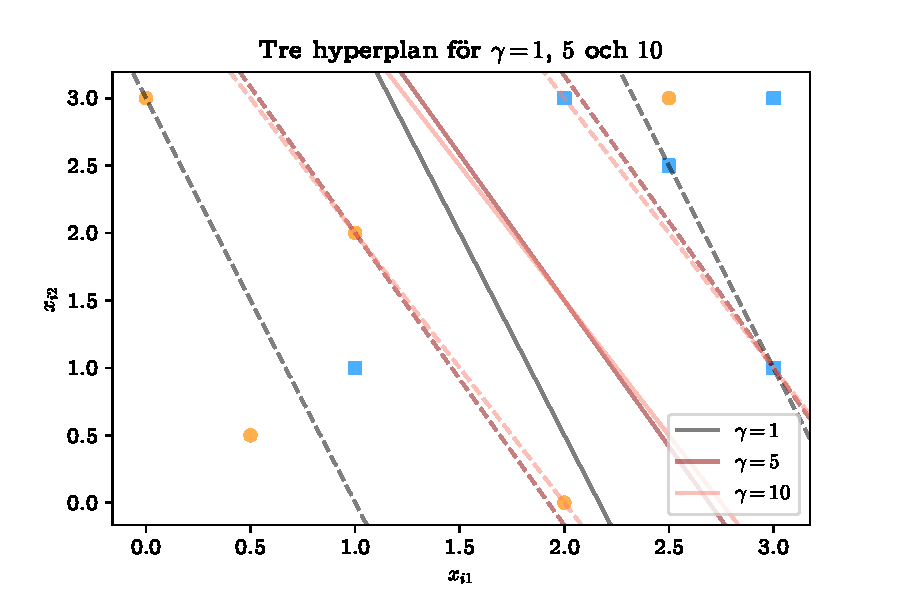
\includegraphics[width=0.8\linewidth, trim={0.5cm 2mm 0.5cm 6mm}, clip]{KandFigur2.pdf}
	\caption{\label{fig:mjukamarginaler}Löst exempel för linjärt oseparabelt data för 3 olika värden på $\gamma$.}
\end{figure}
Låt observationsparen $\left(\mathbf{x}_i,~y_i\right)$ vara sådana som i figur \ref{fig:mjukamarginaler} där blåa rutor är klassen $y_i=1$ och orangea cirklar är klassen $y_i=-1$. Axlarna motsvarar här $\mathbf{x}_i$:s första respektive andra komponenter. Klart är här att observationsparen inte är linjärt separabla men det verkar som att en punkt från vardera klassen kanske mätts fel. För att bestämma en klassificeringsregel används metoden med hyperplan med mjuka marginaler för 3 olika värden på $\gamma$. Funktionen \texttt{SVC} med \texttt{kernel='linear'} från paketet \texttt{sklearn} \cite{sklearn} användes för att beräkna hyperplanen.

Observera hur parametern $\gamma$ påverkar lösningen. Ju mindre $\gamma$ är desto större marginaler vilket betyder att flera punkter används som stödvektorer.
\end{ex}
\begin{ex}\label{ex:olinjär}
\begin{figure}[h]
	\centering
	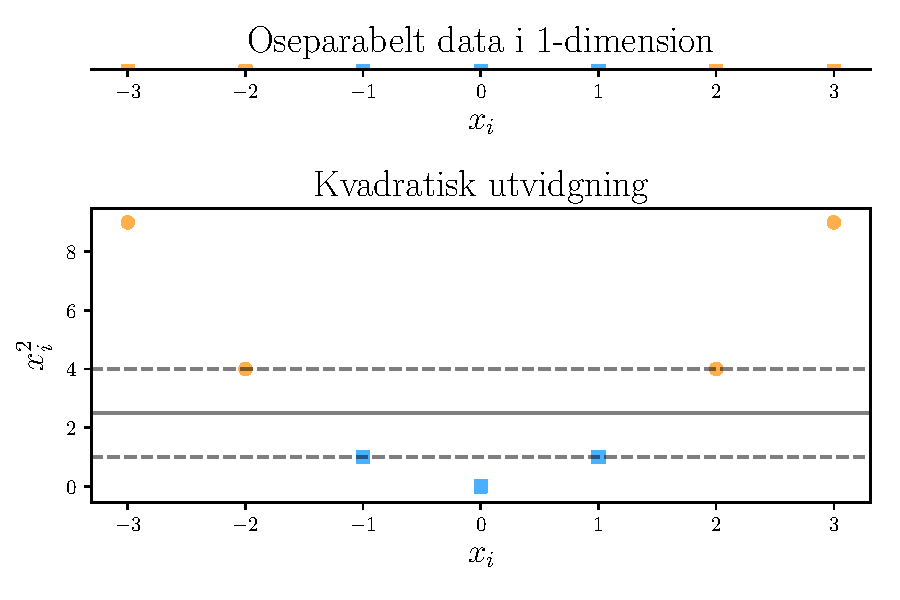
\includegraphics[width=0.8\linewidth, trim={0.5cm 4mm -5mm 4mm}, clip]{KandFigur3.pdf}
	\caption{\label{fig:kvadratisk}En lösning med optimala separerande hyperplan och kvadratisk utvidgning där endast hyperplan med mjuka marginaler inte hade fungerat.}
\end{figure}
Låt $\mathbf{x}_i\in\mathbb{R}$ och observationsparen $\left(\mathbf{x}_i,~y_i\right)$ vara sådana att klassen $y_i=1$ befinner sig mitt i klassen $y_i=-1$, situationen finns illustrerad överst i figur \ref{fig:kvadratisk}. Klart är även här att observationsparen är linjärt oseparabla men nu kan inte heller metoden med hyperplan med mjuka marginaler ge vettiga lösningar. Istället kan man lägga till en dimension och definiera att $\mathbf{x}_i\in\mathbb{R}^2$ och $\mathbf{x}_{i2} = \mathbf{x}_{i1}^2$.
Då får man situationen som illustreras nederst i figur \ref{fig:kvadratisk} och observationsparen är nu linjärt separabla. Det optimala separerande hyperplanet bestämdes med hjälp av \texttt{sklearn}:s metod \texttt{SVC} med \texttt{kernel='linear'} och \texttt{C=1000} \cite{sklearn}.

Moralen här är då att hyperplan med mjuka marginaler inte alltid räcker till utan flera verktyg behövs. Ett sådant verktyg är olinjära utvidgningar av det ursprungliga rummet $\mathbf{x}_i\in \mathbb{R}^p$ till ett större rum där det kan vara enklare att hitta vettiga klassificeringsregler.
\end{ex}
%\FloatBarrier
\chapter{Hilbertrumteori, reproducerande kärnor}\label{chap:hilbert}
Exempel \ref{ex:olinjär} antyder att det kunde vara en bra idé att utvidga observationerna $\mathbf{x}_i$ med olinjära faktorer, frågan är bara hur detta görs bäst. Klart är att man alltid kan bilda $n$:te gradens polynom men ifall den ursprungliga dimensionen $p$, mängden observationspar $N$ eller graden $n$ är stor så kan detta bli övermäktigt för även den snabbaste datorn. Det kommer att visa sig att eftersom observationerna $\mathbf{x}_i$ endast förekommer i inreprodukter (se till exempel korrolarium \ref{cor:inreproduktoptimering} och \ref{cor:mjukinreproduktoptimering}) så finns det ett behagligare alternativ.

\section{Grundläggande teori}
Först några grundläggande definitioner angående \emph{Hilbertrum}, $\mathcal{H}$, det vill säga \emph{fullständiga} vektorrum $X$ försedda med en \emph{inreprodukt} $\langle \cdot , \cdot \rangle$.

\begin{defi}
En \emph{inreprodukt} är en funktion $\langle \cdot , \cdot \rangle: X\times X \longmapsto \mathbb{R}$ sådan att, för alla $\mathbf{x},~\mathbf{y},~\mathbf{z}~\in X$ och alla $\lambda \in \mathbb{R}$, gäller:
\begin{enumerate}
\item $\inprod{x}{y} = \inprod{y}{x}$
\item $\langle \lambda \mathbf{x}, \mathbf{y}\rangle = \lambda \inprod{x}{y}$
\item $\inprod{x+y}{z} =\inprod{x}{z} + \inprod{y}{z}$
\item $\inprod{x}{x} \geq 0$, där likhet gäller om och endast om $\mathbf{x} = \mathbf{0}$. 
\end{enumerate}
\end{defi}
\begin{defi}
Ett vektorrum $X$ är \emph{fullständigt} om varje Cauchyföljd $\mathbf{x}_n$ konvergerar till en punkt $\mathbf{x}\in X$.
\end{defi}

\begin{rem}
Dimensionen på vektorrummet $X$ nämns inte i definitionen för inreprodukten och därför kan Hilbertrum även vara oändligtdimensionella. Många av de bekanta egenskaperna för ändligtdimensonella inreproduktrum gäller även för oändligtdimensionella inreproduktrum, till exempel är två vektorer $\mathbf{x}, ~\mathbf{y}$ ortogonala ifall $\inprod{x}{y}=0$, även om det kan vara svårt att visualisera för oändligtdimensionella rum.
\end{rem}
På tal om ortogonalitet så vore det behändigt att ha någon parallell till de ändligtdimensionella vektorrummens koordinatsystem och basvektorer. Det visar sig att inte alla Hilbertrum har en motsvarighet till basvektorer men ifall man kräver att rummet är \emph{separabelt} så existerar en ortonormal följd vektorer $\mathbf{e}_i$ sådan att för varje vektor $\mathbf{x}\in \mathcal{H}$  gäller \cite{Young}:
\begin{equation*}
	\mathbf{x}=\sum_{i=1}^{\infty}\left\langle \mathbf{x}, \mathbf{e}_i \right\rangle \mathbf{e}_i
\end{equation*}
där vektorerna $\mathbf{e}_i$ agerar bas och koefficienten $\left\langle \mathbf{x}, \mathbf{e}_i \right\rangle$ kallas den $i$:te Fourierkoefficienten med avseende på basen $\mathbf{e}_i,$ $i=1,2,3,\dots$. I fortsättningen behandlas bara separabla Hilbertrum, så att varje vektor $\mathbf{x}$ kan skrivas som en linjär kombination av basvektorerna.

Elementen i Hilbertrummen kan också ha många olika former, till exempel de $d$-dimensionella vektorerna med den vanliga inreprodukten $\left\langle \mathbf{x}, \mathbf{y} \right\rangle = \mathbf{x}^\intercal\mathbf{y}$ som hittills behandlats. Man kan även tillåta att elementen är funktioner, till exempel på intervallet $\left[a,b\right]$, då brukar inreprodukten definieras som
\begin{equation*}
	\left\langle f, g \right\rangle=\int_{a}^{b}f(x)g(x) dx,
\end{equation*}
men man måste dessutom kräva att normen $\left\|f\right\| = \left(\int_{a}^{b}f(x)^2dx\right)^{\frac{1}{2}}$ är ändlig för alla funktioner i rummet.

Speciellt när det kommer till Hilbertrum med funktioner som element, så kallade \emph{funktionsrum}, så behandlar man \emph{funktionaler} istället för funktioner för att undvika förvirring.
\begin{defi}
	En \emph{funktional} $\mathcal{F}$ är en reellvärd funktion som tar en annan funktion $f$ som argument, det vill säga
	\begin{equation*}
		\mathcal{F}: \mathcal{H} \longmapsto \mathbb{R}
	\end{equation*}
	där elementen i Hilbertrummet $\mathcal{H}$ är funktioner.
\end{defi}

En funktional är linjär om följande gäller:
\begin{equation*}
	\mathcal{F}(\lambda f+g) = \lambda\mathcal{F}(f) + \mathcal{F}(g),
\end{equation*}
för alla $f$, $g$ $\in \mathcal{H}$, $\lambda \in \mathbb{R}$ och \emph{begränsad} om följande gäller:
\begin{equation*}
	\sup \left\{\left| \mathcal{F}(u) \right| : u\in\mathcal{H},~\left\| u \right\|_{\mathcal{H}} \leq 1 \right\} < \infty
\end{equation*}
där $\left\| \cdot \right\|_ \mathcal{H}$ är den inducerade normen i Hilbertrummet $\mathcal{H}$.

Dessutom gäller att linjära funktionaler är begränsade om och endast om de är kontinuerliga. Det gäller även att funktionaler är kontinuerliga om och endast om de är kontinuerliga i 0 \cite{Young}.

Följande sats ger ett sätt att karaktärisera varje begränsad linjär funktional $\mathcal{F}$ som en inreprodukt.

\begin{thm}[Riesz-Fréchets representations sats \cite{Young}]
	För varje begränsad linjär funktional på ett Hilbertrum $\mathcal{H}$, $\mathcal{F}: \mathcal{H} \longmapsto \mathbb{R}$, existerar ett unikt $v\in\mathcal{H}$ sådant att
	\begin{equation}
		\mathcal{F}(u)=\left\langle u, v\right\rangle_\mathcal{H}\quad \text{för alla }u\in\mathcal{H}
	\end{equation}
	för alla $u\in\mathcal{H}$, där $\left\langle \cdot, \cdot\right\rangle_\mathcal{H}$ betecknar inreprodukten i Hilbertrummet $\mathcal{H}$.\\
	Dessutom gäller att $\left\| v \right\|_\mathcal{H}=\left\| \mathcal{F}\right\|_O$ där $\left\| \cdot \right\|_\mathcal{H}$ är den inducerade normen och $\left\|\cdot\right\|_O$ är operatornormen \begin{equation*}
	\left\|\mathcal{F}\right\|_O:=\sup_{u\in\mathcal{H},\left\|u\right\|_\mathcal{H}\leq 1}\left|\mathcal{F}(u)\right|.
	\end{equation*}
\end{thm}
\begin{proof}
	Nedan följer en översikt av beviset i \cite{Young}.
	
	Ifall $\mathcal{F}$ är funktionalen som avbildar varje element $u\in\mathcal{H}$ på 0 så är satsen bevisad genom att man väljer $v=0$. 
	
	Antag att det existerar åtminstone ett $u\in\mathcal{H}$ sådant att $\mathcal{F}(u)\neq0$. Då kan man dela upp $\mathcal{H}$ i två delar,
	\begin{equation*}
		\mathcal{M} = \left\{u\in\mathcal{H}:\mathcal{F}\left(u\right)=0\right\}
	\end{equation*}
	och
	\begin{equation*}
		\mathcal{M}^\perp = \left\{u\in\mathcal{H}: \left\langle u,w \right\rangle=0\text{ för alla }w \in \mathcal{M}\right\},
	\end{equation*}
	det vill säga $\mathcal{M}^\perp$ är det \emph{ortogonala komplementet} till $\mathcal{M}$.
	Då gäller att varje element $w_0\in \mathcal{H}$ kan skrivas som summan $w_0 = w_1 + w_2$ där $w_1\in\mathcal{M}$ och $w_2\in \mathcal{M}^\perp$ (Sats 4.24 i \cite{Young}). Lineariteten av $\mathcal{F}$ ger då att $\mathcal{F}(w_0)=\mathcal{F}(w_1)+\mathcal{F}(w_2)=\mathcal{F}(w_2)$, på grund av detta och antagandet att det existerar ett $w_0\in\mathcal{H}$ sådant att $\mathcal{F}(w_0)\neq0$ måste det finnas åtminstone ett element $w_2 \neq 0$ i $\mathcal{M}^\perp$. Välj $x:= \frac{w_2}{\mathcal{F}(w_2)}$, då är $\mathcal{F}(x)=\mathcal{F}\left(\frac{1}{\mathcal{F}(w_2)}w_2\right)=\frac{\mathcal{F}(w_2)}{\mathcal{F}(w_2)}=1$ och $x\in\mathcal{M}^\perp$.
	För varje element $u\in\mathcal{H}$ kan man då skriva
	\begin{equation*}
		u=\underbrace{\left(u-\mathcal{F}(u)x \right)}_{\in\mathcal{M}} + \underbrace{\mathcal{F}(u)x}_{\in \mathcal{M}^\perp}.
	\end{equation*}
	Om man sedan tar inreprodukten med $x$ på båda sidorna så får man
	\begin{align*}
		\left\langle u,x \right\rangle &= \underbrace{\left\langle u-\mathcal{F}(u)x ,x \right\rangle}_{=0} + \left\langle \mathcal{F}(u)x,x \right\rangle\\
		&= \mathcal{F}(u)\langle x, x\rangle=\mathcal{F}(u)\|x\|^2
	\end{align*}
	eftersom att $u-\mathcal{F}(u)x\in\mathcal{M}$ och $\langle w, x \rangle=\langle x,w\rangle=0$ för alla element $w\in \mathcal{M}$ då $x\in\mathcal{M}^\perp$. Om man då väljer $v=\frac{x}{\|x\|^2}$ får man att
	\begin{align*}
		\langle u,v \rangle &= \left\langle u , \frac{x}{\|x\|^2}\right\rangle= \frac{\langle u, x\rangle}{\|x\|^2}\\
		&= \frac{\mathcal{F}(u)\|x\|^2}{\|x\|^2}\\
		&= \mathcal{F}(u)
	\end{align*}
	och då är den första delen av satsen bevisade. Den andra delen är inte lika intressant i detta fall så beviset lämnas bort.
\end{proof}

\section{Reproducerande Kärnor}
Betrakta funktionen $\Phi:(x)\longmapsto (x^2,\sqrt{2}x, 1)$ där $x\in\mathbb{R}$, denna funktion motsvarar den olinjära utvidgningen i exempel \ref{ex:olinjär}. För att lösa exempel \ref{ex:olinjär} borde följande inreprodukt mellan två observationer $\mathbf{x}_1$ och $\mathbf{x}_2$ beräknas:
\begin{align*}
	\left\langle \Phi(\mathbf{x}_1), \Phi(\mathbf{x}_2) \right\rangle_3 &= \bfx_1^2\bfx_2^2 + 2\bfx_1\bfx_2 + 1\\
	&= \langle \bfx_1, \bfx_2 \rangle_1^2 + 2\langle \bfx_1, \bfx_2 \rangle_1 + 1\\
	&= \left(\langle\bfx_1, \bfx_2 \rangle_1 + 1\right)^2 = k(\bfx_1, \bfx_2)
\end{align*}
där $\langle \cdot, \cdot \rangle_d$ är den vanliga inreprodukten i $\mathbb{R}^d$.

Funktioner $k(\bfx_1, \bfx_2)$ som kan uttryckas som en inreprodukt av en funktion $\Phi$ evaluerad i två olika punkter $\bfx_1$ och $\bfx_2$ brukar kallas \emph{kärnor} och studerades först av David Hilbert \cite{Hilbert} i samband med studien av integraloperatorn $T_k f(x)=\int_{X}k(x_1, x_2)f(x_2)dx_2$ där funktionen $k$ är operatorn $T_k$:s kärna \cite{LearningKernels}.



Bygg vidare på korrolarium \ref{cor:mjukinreproduktoptimering}:s mjuka motsvarighet genom att byta ut inreprodukten mot en annan, ge krav på inreprodukten. Visa att just precis de inreprodukter som samtidigt är reproducerande kärnor uppfyller de kraven.

(Bevis av Mercers villkor för positivsemidefinita ekvationer/operatorer, behöver åtminstone Riesz representationssats och någon sats om eigenvärden/funktioner, material från kursen fördjupad analys I/II borde "räcka". Måste kanske hoppa över vissa tekniska detaljer.)

\chapter{Avslutning}
Har hittills inte gått in på statistiska detaljer, till exempel tränings/validerings-data eller gränser på felklassificering.

Kan också nämna andra varianter som till exempel användning inom regression, "glesa" (sparse) varianter.

\bibliographystyle{sweplain}
\bibliography{bibliografi}
\end{document}
